\chapter{Preliminary Machine Learning Experiments}
\label{cha:preliminary}

This chapter covers work which was completed as part of research for this PhD project, but were not included as part of a journal article. They include preliminary experiments, negative results and other exploratory research. 

\section{Dataset Size Sensitivity}

\noindent The motivation for this experiment was not to investigate the effectiveness of a particular method or approach, but rather to determine the sensitivity of model performance to data-set size. \\

\noindent From the larger data-set, 6000 cases  were randomly chosen. This set was split into 6 segments of equal size. The experimental procedure involved incrementally adding the segments to data-set used to train the model. After the adding of of each increment to the training data-set, the model was reinitialised with random starting weights so training could begin afresh. This process was repeated four times to account for the stochastic nature of the model initialisation process. \\

\noindent At each stage of the experiment, the data-set was randomly split into a training set (80\% of instances) and validation set (the remaining 20\%). The model architecture and parameters were kept constant for all increments of data-set size. The model used was a convolutional neural network, with 8 convolutional layers, each 64 nodes wide and 2 fully connected layers before the output layer. 
\\

\noindent 
Figure~\ref{fig:sensitivity_summary} gives a summary of the results for the experiment. Each pair represents a increment of the experiment, with the blue and orange bars representing the average training and validation loss at the end of the training process. As can be seen, the training loss after the final epoch is very similar in each increment. The average validation result, however, falls with each increase in the size of the data-set. \\

\noindent Looking more closely at the training process, we can examine the training loss history for each increment. Figure~\ref{fig:history_1000} shows that for a data-set size of 1000 instances, the training loss falls steadily, however, the validation rises steadily for the first 100 epochs and then converges. These seems to suggest the model is over-fitting with a data-set of this size. \\

\noindent When the data-set is increased in size to 3000 (Figure~\ref{fig:history_3000}), the training loss steadily decreases except for a spike at epoch 150. Similar behaviour can be seen for the validation loss, however, it appears to converge at around 200 epochs. Increasing the data-set size to 5000 (Figure~\ref{fig:history_5000}), validation loss convergence occurs at a lower loss value. Additionally, the training and validation losses at the end of training are closer to one another.
\\

\begin{figure}[b]
	\centering
	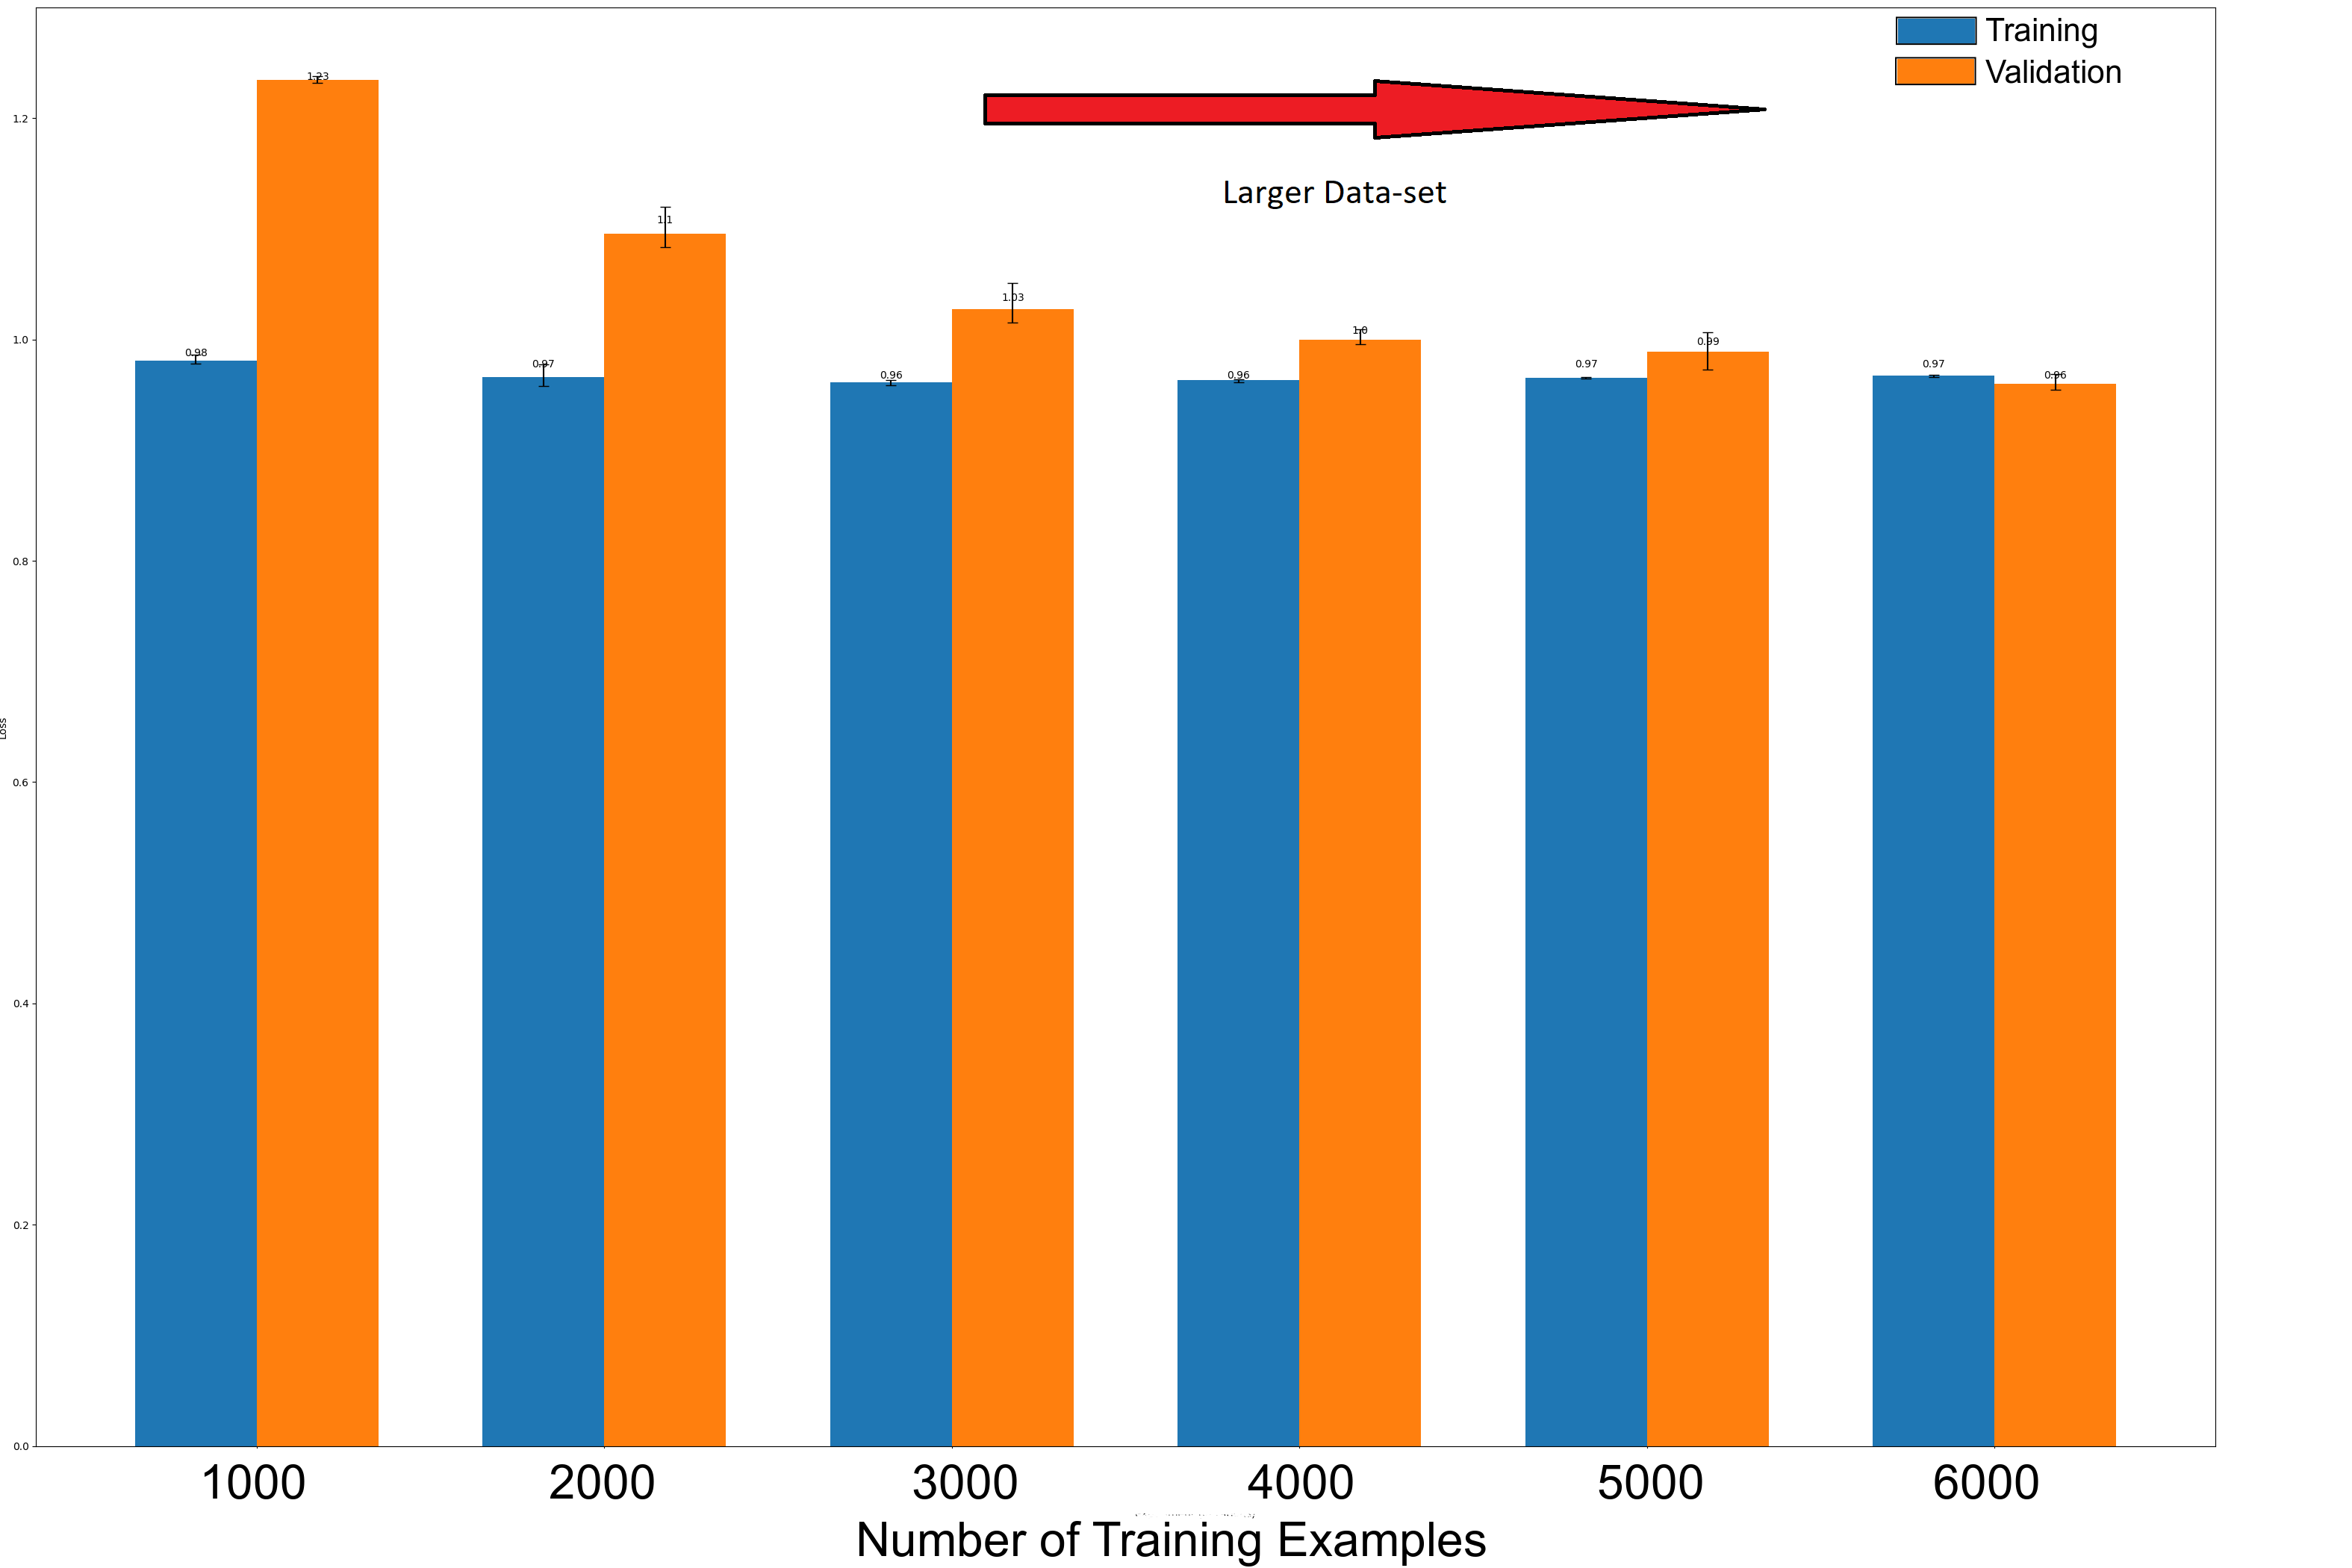
\includegraphics[scale=0.14]{Figures/comparing_models_Sensitivity.png}
	\caption{Sensitivity Results Summary}
	\label{fig:sensitivity_summary}
\end{figure}

\begin{figure}[b]
	\centering
	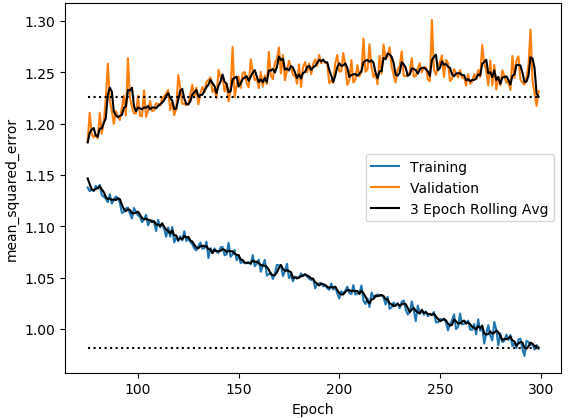
\includegraphics[scale=0.75]{Figures/TrainHistory_dataset_cases1000_C0_321_L0_13_0_321_0_13_48_1_allI0.png}
	\caption{Training History of Increment with a Data-set of 1000 Increments}
	\label{fig:history_1000}
\end{figure}

\begin{figure}[b]
	\centering
	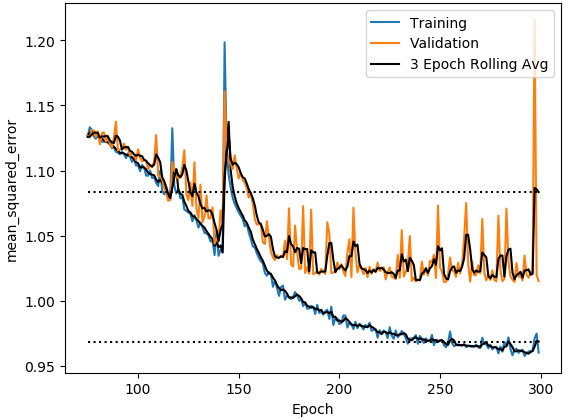
\includegraphics[scale=0.75]{Figures/TrainHistory_dataset_cases3000_C0_321_L0_13_0_321_0_13_48_1_allI0.png}
	\caption{Training History of Increment with a Data-set of 3000 Increments}
	\label{fig:history_3000}
\end{figure}

\begin{figure}[b]
	\centering
	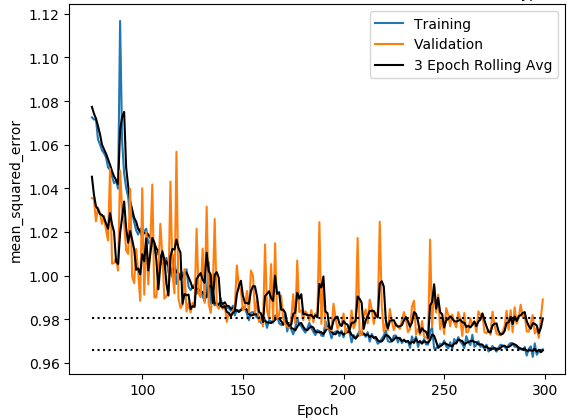
\includegraphics[scale=0.75]{Figures/TrainHistory_dataset_cases5000_C0_321_L0_13_0_321_0_13_48_1_allI0.png}
	\caption{Training History of Increment with a Data-set of 5000 Increments}
	\label{fig:history_5000}
\end{figure}

\noindent
It's clear from this experiment that a larger data set yields improved results. This result is as would be expected - a larger dataset yields more training examples for the model to learn from and reduces the potential for overfitting~\cite{hawkins2004problem}.  Looking carefully at Figure~\ref{fig:sensitivity_summary}, we can see performance improves sharply for the first two increments. Following this, we have diminishing returns, with the final two incremental increases in dataset size yielding only very small improvements in model performance.  This suggests that at 6000 samples,  the training dataset is reaching a point of saturation i.e. increasing the size of the dataset much further is unlikely to yield significant model performance. The results of this experiment implies that we should focus computational and research efforts into machine learning model refinement rather than generating more Parmec data. However, investigations of increasing the dataset by a significant amount, say by an order of magnitude, should be investigated at a later date. This may be possible through techniques such as data augmentation \cite{shorten2019survey}.


\section{Crack Orientation}

Recall from subsection~\ref{data:inputs} that our input feature matrix can be represented by $\textbf{X} = \{-1, 1\}^{N \times BF}$, with N being the number of training samples and BF being the number of fuel bricks in the Parmec model. Each element in this matrix is either a -1 (representing an uncracked brick), or a 1 representing a cracked brick. 
\\

\noindent
Note also that in subsection~\ref{data:inputs} it was discussed that Parmec can represent a cracked fuel brick in one of four orientations (see Figure~\ref{fig:orientations}). In the format of the input feature matrix discussed in the previous paragraph, the orientation of a cracked brick is not encoded and this information is discarded. 
\\

\noindent
If we wish to encode this information for the purposes of  developing a machine learning model, how we go about this? We could adapt our input feature matrix to the form $\textbf{X} = \{-1, 4\}^{N \times BF}$ so that a cracked brick is denoted by a 1 - 4 inclusive, representing one of the crack orientations shown in Figure~\ref{fig:orientations}. However, a machine learning model would treat these as ordinal values i.e. it would see orientation 2 as being double that of orientation 1. Effectively there is no ordinal relationship between the orientations and so this format would be incorrect.\\ 

\noindent
Instead, our feature matrix is expanded into an extra dimension. As opposed to a 0 or 1 for each brick representing an uncracked or cracked brick, each brick is now represented by a vector of length 4. An uncracked brick is represented by a vector of four zeros, with each crack orientation (Figure~\ref{fig:orientations}) represented by a 1 in one of the four vector elements (\ref{one_hot}).
\\

\begin{equation} \label{one_hot}
	\textbf{Uncracked} = \{0, 0, 0, 0\}  \notag
\end{equation}
\begin{gather}
	\textbf{Orientation 1} = \{1, 0, 0, 0\}  \notag
\end{gather}
\begin{align}
	\textbf{Orientation 2} = \{0, 1, 0, 0\} 
\end{align}
\begin{align}
	\textbf{Orientation 3} = \{0, 0, 1, 0\}  \notag
\end{align}
\begin{align}
	\textbf{Orientation 4} = \{0, 0, 0, 1\}  \notag
\end{align}

\noindent This approach is functionally similar to one-hot encoding \cite{seger2018investigation}, where categorical values are represented by a binary vector. \\

\noindent
In this experiment, two machine learning models were trained in parallel: the first using our original input feature encoding ($\textbf{X} = \{-1, 4\}^{N \times BF}$) and the second with our expanded input feature tensor which encodes cracked brick orientation \ref{one_hot}. In both parts of the experiment, the model architecture and all other parameters were kept constant.  The training and evaluation process was repeated four times per input encoding format, so as to account for the stochastic nature of hyper-parameter initialisation.
\\

\noindent It was expected that the model trained using the expanded input feature tensor would outperform  the model trained using binary encoding.  After all, it is the same experiment except for the additional information of crack orientations as well as positions. However, only a very similar performance was seen, or in some cases, slightly worse. It appears that the model training process exhibits overfitting - where the model too closely fits the training set, including any noise or irrelevant information.  A clear indicator of overfitting is decreasing training loss whilst validation loss increases i.e. the model fits to the training set so well that it losses the ability to generalise to data outside of it. Looking at the training time history of the model trained using crack orientations, this phenomenon can be clearly seen in (Figure~\ref{fig:history_ori}). It can be seen that the training loss falls monotonically, with the validation loss rising steadily i.e. the model's ability to generalise is falling. \\

\noindent There are several explanations for the unexpectedly lower performance of the model trained with the input features including orientations. The first possibility is that the positions of the cracks is the overriding factor of importance in terms of causing displacements, with the orientations having little physical effect. The other possibility is that the results are an artefact of the way they have been encoded or expressed to the model. Further study should be made to investigate this at a later time.

\begin{figure}[!ht]
	\centering
	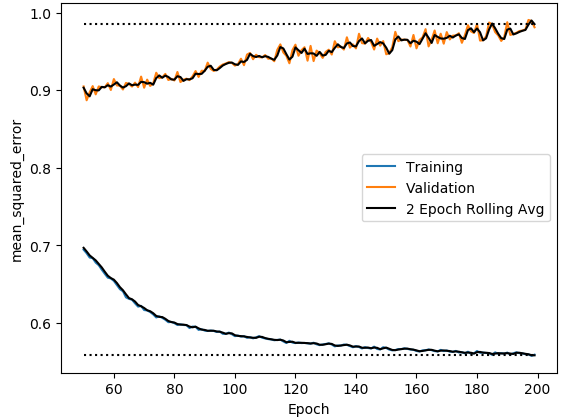
\includegraphics[scale=0.7]{Figures/train_history_ori.png}
	\caption{Training History for Crack Orientation Model }
	\label{fig:history_ori}
\end{figure}

\section{Transfer Learning}


As outlined in subsection~\ref{transfer}, existing models for image classification can be adapted to other problems, including the regression problem of this research work. Models from the VGG and ResNet families were adapted, including VGG16 \& VGG19 and ResNet50 \& ResNet101. These were trained and tested using the standard data-sets used previously. It was found that VGG19 performed the best out of all of these methods, with VGG16 also performing better than all ResNet models.
\\

\noindent
To suit the purpose of this study, the existing models had to be adapted. Previously, these models would receive a image tensor, usually of dimensions 32x32x3 (32 pixels width and depth plus 3 colour channels) and output a vector of length 1000 (representing a range of image categories). In place of the image tensor, the 3-dimensional tensor represented by Figure~\ref{fig:cascade} was flattened into a planar arrangement with an example shown in Figure~\ref{fig:transfer_encoding}. This was then one-hot encoded into three channels: cracked bricks (green), uncracked bricks (red) and corners/edges (blue). For each instance, this processes creates a input feature tensor of 88x44x3. The model output layer was modified to produce a single regression value.  
\\

\begin{figure}[h]
	\centering
	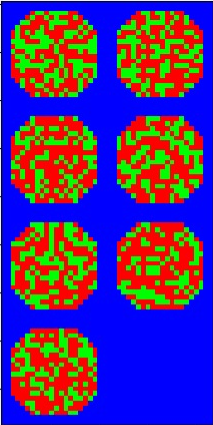
\includegraphics[scale=0.75]{Figures/vgg_encoding.png}
	\caption{Feature encoding appropriate for use in transfer learning} {This image shows a single Parmec instance encoded in a planar configuration.}
	\label{fig:transfer_encoding}
\end{figure}

\noindent
This experiment also involved adding layers between the end of the nominal VGG19 architecture and the output layer. These included dropout layers of varying percentages, dense layers of varying width and batch normalisation layers [\cite{liao2016importance}]. The summary of results can be seen in Table~\ref{tab:exp3}. It can be seen that simply adding a dropout layer of 30\% results in the best model performance uplift, with some adding reducing performance. A visualisation of the model performance can be seen in Figure~\ref{fig:results_transfer}. 

\begin{table}[h!]
	\begin{center}
		
		\begin{tabular}{c|c|c|c} % <-- Alignments: 1st column left, 2nd middle and 3rd right, with vertical lines in between
			\textbf{Additional} & \textbf{Additional} & \textbf{Additional} & \textbf{Lowest} \\
			
			\textbf{Layer 1} & \textbf{Layer 2} & \textbf{Layer 3} & \textbf{Loss} \\
			\hline
			Dropout 30\% & - & - & 7.8e-2  \\
			Dropout 40\% & - & - & 7.9e-2  \\ 
			(none) & - & - & 7.9e-2  \\
			Batch Norm & Dense (32) & Dropout 20\% & 8.0e-2  \\
			Dense (32) & Dropout 20\% & Dense (16) & 8.1e-2  \\
			Dense (32) & Dropout 30\% & Dense (32) & 8.2e-2  \\
		\end{tabular}
		\caption{Summary of the Test Results from Preliminary Transfer Learning Experiment}
		\label{tab:exp3}
	\end{center}
\end{table}

\noindent
It was also mentioned in subsection~\ref{transfer} that the option exists in transfer learning to import existing weights optimised for the original purpose of the model, or to start with fully randomised starting weights. It was found here that using the ImageNet weights as a starting point for the model significantly improved model performance, both in terms of time to convergence and overall loss.

\begin{figure*}[p]
	\centering
	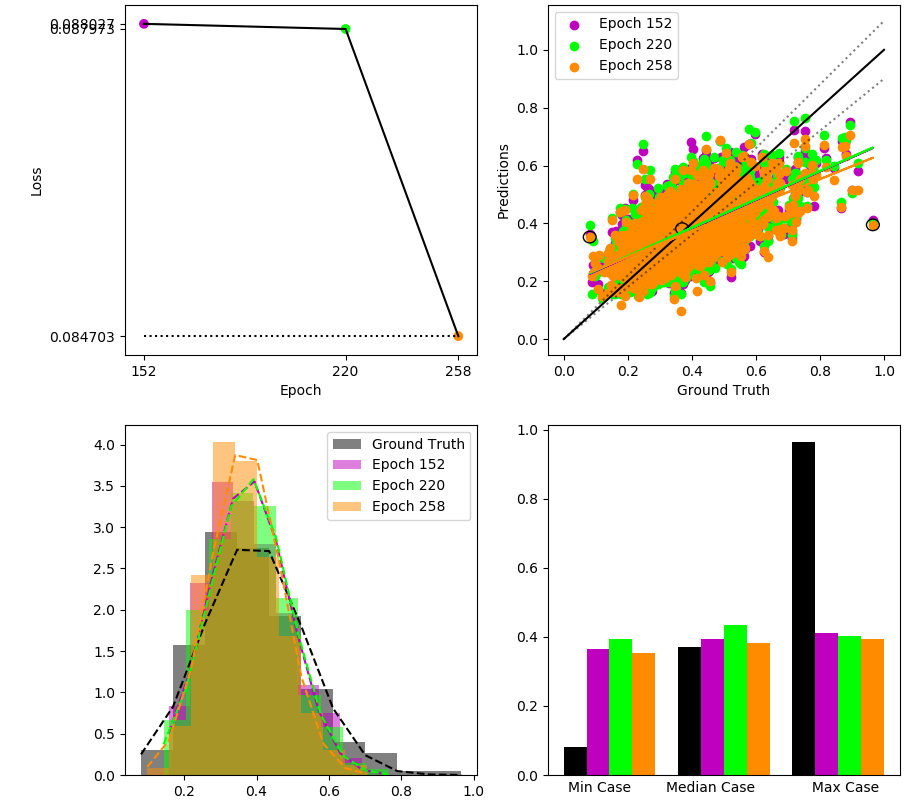
\includegraphics[scale=0.7]{Figures/transfer3.png}
	\caption{Results Dashboard for VGG19 Model with added Dropout Layer (30\%).}
	\label{fig:results_transfer}
\end{figure*}

\noindent
Over all, the transfer learning models produced inferior results to those of an architecture developed from scratch. However, the transfer learning models still provided comparable results and may have superior results in some parts of the data-range, particularly the lower part.

\section{Whole Core Experiment} \label{prelim:whole}

As mentioned in subsection~\ref{data:outputs}, the output of Parmec is multi-dimensional, with 6 directional/rotational outputs for all 4173 interstitial bricks, with each of these values output at all 271 time frames during the earthquake. In this experiment, a single time frame was selected (frame 48) and one output metric (displacement in the West-East direction). The rationale for selecting these outputs starts by examining and comparing Figures~\ref{fig:results1} \& \ref{fig:results2}, as well as Figures~ref{fig:histo1} \& ref{fig:histo1}. Displacement in the South-North direction was discarded as limited variability can be seen looking at individual cases and at the distribution of the dataset as a whole. Looking at individual cases of displacement in the West-East direction, it can be seen that there is variability between cases (top row of Figure~\ref{fig:results1}). Also, there are a reduced number of outliers (Cyan in Figure~\ref{fig:histo1}) compared to outputs for the other time frames. 
\\

\noindent
With our selection of output data, a machine learning model was trained for 200 epochs to predict displacement in the West-East direction at frame 48 for all 4173 interstitial bricks. A visualisation of the test set predictions for a single instance can be seen in Figures~\ref{fig:preds_layer_7} \& \ref{fig:preds_layer_10}. These figures visualise the predictions of the model at the half way point of training and after the final epoch, comparing each to the ground truth.
\\

\begin{figure*}[p]
	\centering
	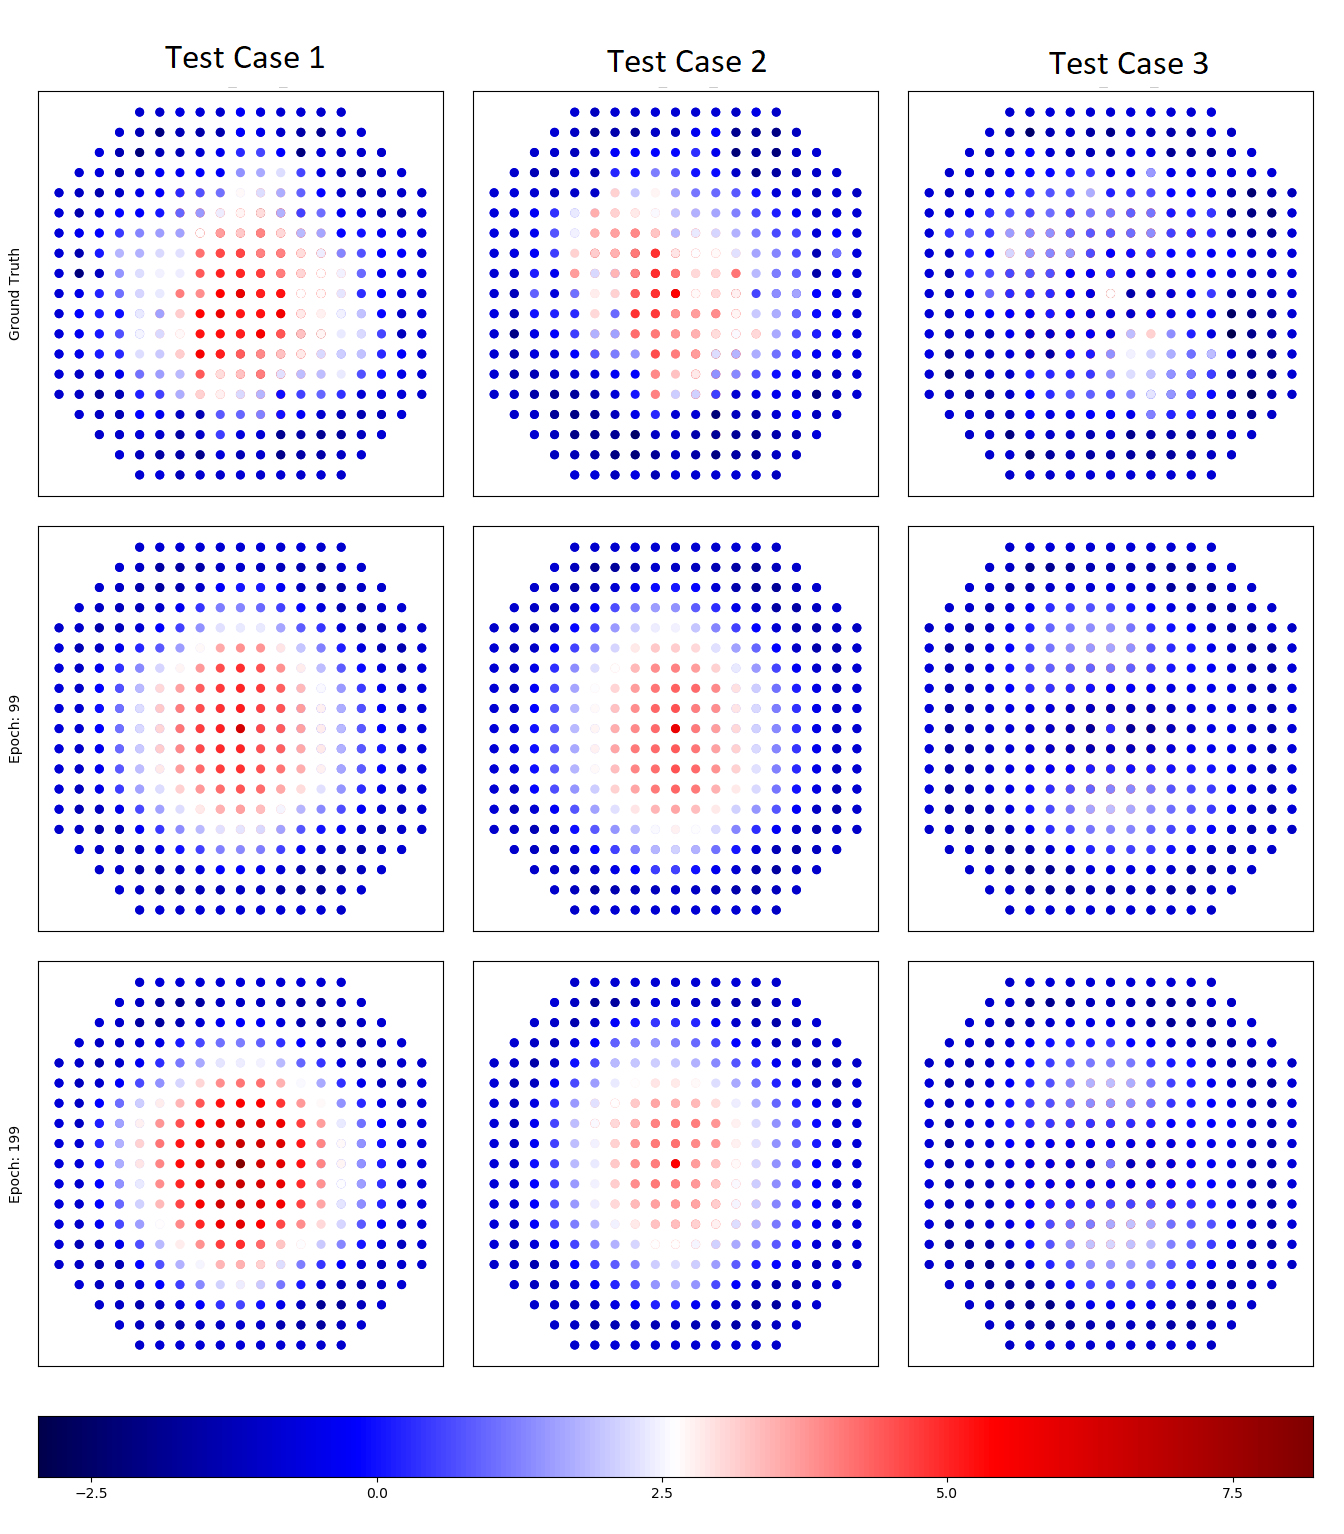
\includegraphics[scale=0.45]{Figures/preds_layer_7.png}
	\caption{Direct comparison of model predictions against ground truth labels for core level 7} {This comparison is made for predictions on the test data-set and at two points during the training process. Each column represents a different example case from the testing data-set. The top row represents the ground truth labels with the two subsequent rows showing the predictions of the model at epoch 100 and 200 (final epoch). }
	\label{fig:preds_layer_7}
\end{figure*}

\begin{figure*}[p]
	\centering
	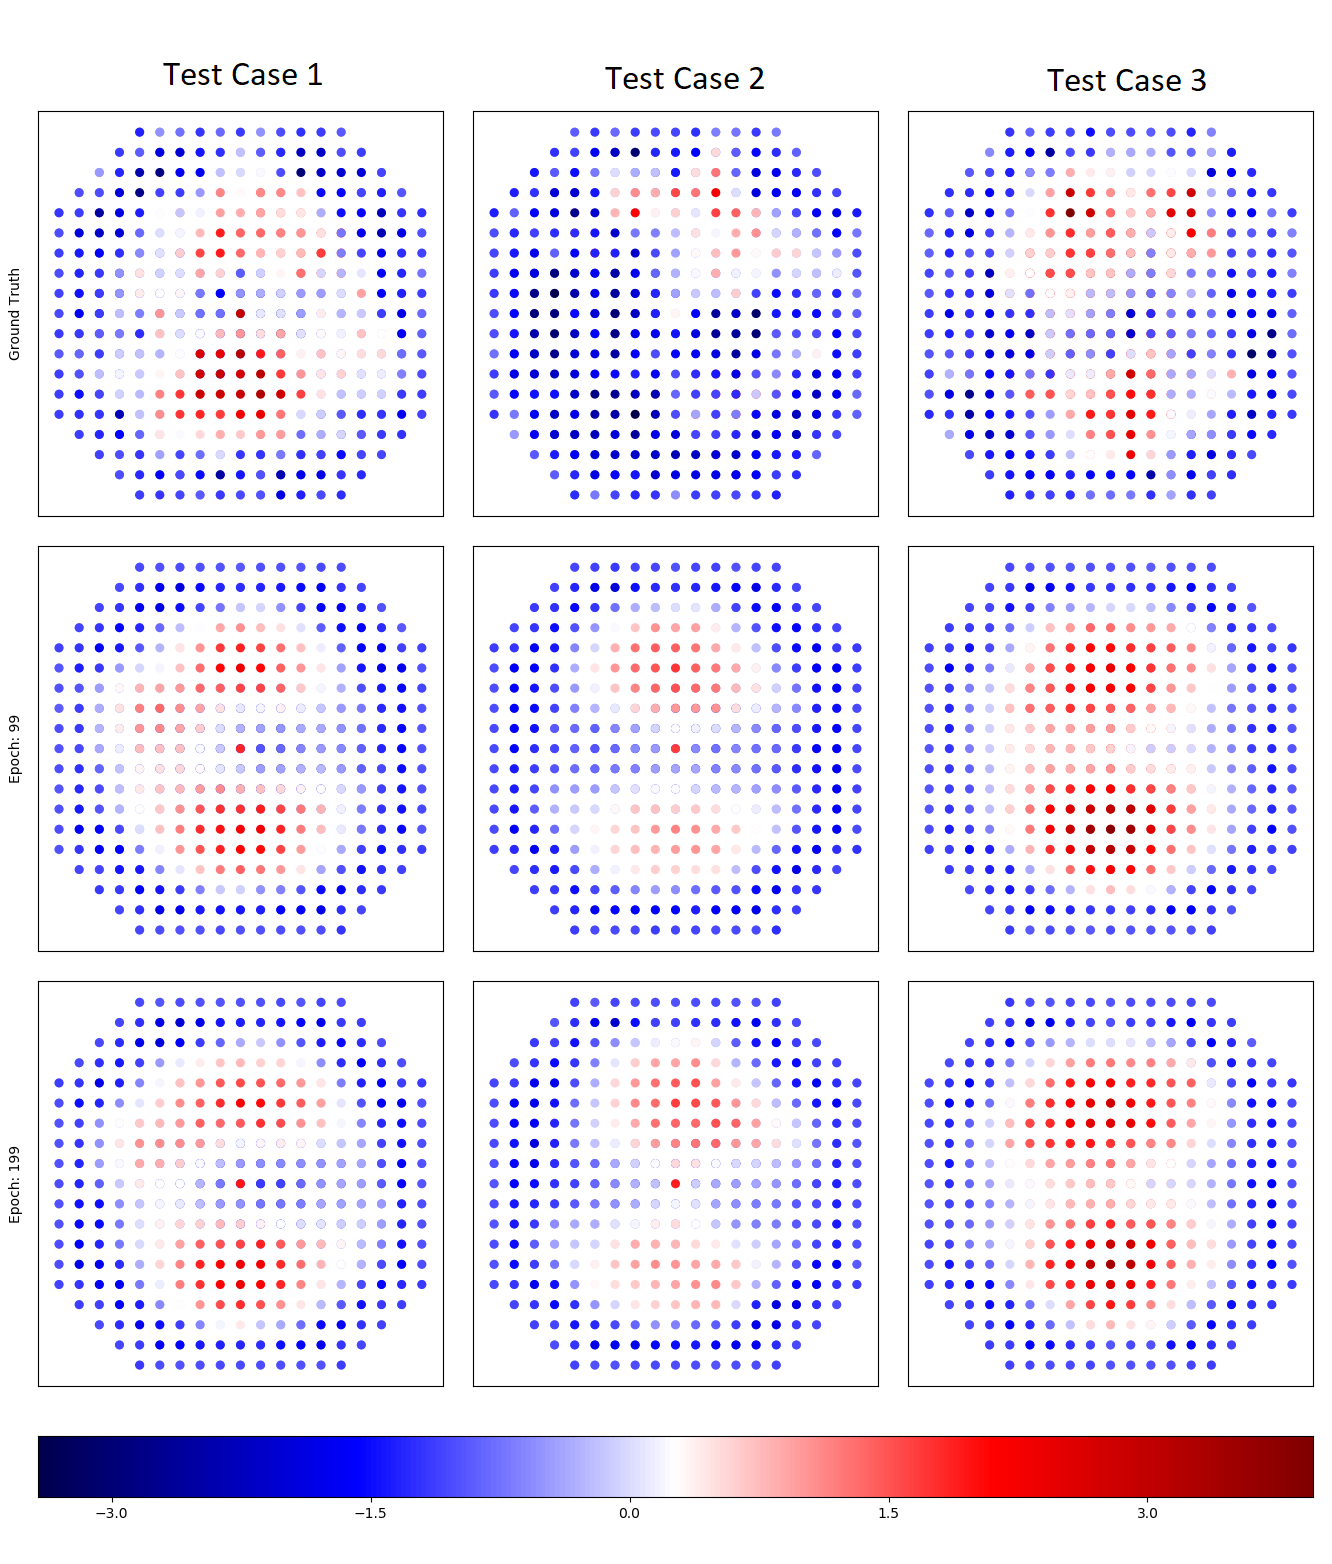
\includegraphics[scale=0.45]{Figures/preds_layer_10.png}
	\caption{Direct comparison of model predictions against ground truth labels for core level 10} {This comparison is made for predictions on the test data-set and at two points during the training process. Each column represents a different example case from the testing data-set. The top row represents the ground truth labels with the two subsequent rows showing the predictions of the model at epoch 100 and 200 (final epoch). }
	\label{fig:preds_layer_10}
\end{figure*}

\noindent
It can be seen that the model makes similar predictions for all three cases i.e. there is limited variability between the predictions. This suggests the model has a high level of bias and is not able to generalise well. The explanation for this can likely be found in the discussion within subsection \ref{correlation}, where it was revealed that the outputs for disparate regions of the core do not correlate well with each other. Therefore, this result suggests that the development of a machine learning model with the intention of predicting the displacement of all 4173 bricks may be highly complex and take considerable effort in model optimisation. Therefore, the development of a model with a narrower output prediction scope first may be a more reasonable short term goal.
